\documentclass[11pt,a4paper]{article}
\usepackage[margin=1in]{geometry}
\usepackage{setspace}
\usepackage{hyperref}
\usepackage{enumitem}
\usepackage{amsmath}
\usepackage{amssymb}
\usepackage{xcolor}
\usepackage{booktabs}
\usepackage{graphicx}
\usepackage{tikz}
\usetikzlibrary{arrows.meta,positioning,shapes,fit,calc}
\usepackage{pgfplots}
\usepackage{titlesec}
\pgfplotsset{compat=1.18}

\setstretch{1.15}
\definecolor{accent}{HTML}{1F77B4}
\definecolor{accent2}{HTML}{FF7F0E}
\definecolor{accent3}{HTML}{2CA02C}
\definecolor{softbg}{RGB}{245,248,252}

\renewcommand{\familydefault}{\sfdefault}

\title{\textbf{Context-Aware FinCommerce Engine\\using Vector Memory with Qdrant}}
\author{}
\date{January 2026}

\titleformat{\section}[block]{\Large\bfseries\color{accent}}{}{0pt}{}
\titleformat{\subsection}[block]{\large\bfseries\color{accent}}{}{0pt}{}
\titleformat{\subsubsection}[block]{\normalsize\bfseries\color{accent}}{}{0pt}{}

\newcommand{\callout}[1]{%
  \vspace{0.4em}%
  \noindent\colorbox{softbg}{\parbox{\dimexpr\linewidth-2\fboxsep}{#1}}}

\newcommand{\badge}[1]{\tikz[baseline=(x.base)]\node[fill=accent!12,draw=accent!60,rounded corners=2pt,inner sep=2.5pt](x){\scriptsize #1};}

\begin{document}

\maketitle
\newpage

\tableofcontents
\newpage

\section{Introduction}

Modern e-commerce platforms face a fundamental challenge: delivering recommendations that are simultaneously \textit{semantically relevant}, \textit{financially feasible}, \textit{personally aligned}, and \textit{behavior-informed}. Traditional keyword-based search systems decouple these dimensions, forcing users to navigate fragmented experiences across search, price filters, trending widgets, and recommendation sidebars.

The problem is not one of retrieval—search engines excel at finding relevant items. Rather, it is one of \textit{contextual synthesis}. Users shopping online operate within multiple constraints and motivations simultaneously:

\begin{itemize}[leftmargin=1.2em]
  \item \textbf{Financial Realities}: Available balance, credit limits, debt obligations, installment eligibility
  \item \textbf{Semantic Intent}: Product specifications, use cases, domain language
  \item \textbf{Personal Preferences}: Trusted brands, favorite categories, style preferences
  \item \textbf{Social Proof}: What similar users purchased, trending items in real-time
\end{itemize}

Vector databases like Qdrant enable a fundamentally different paradigm: \textit{vector-native memory}. Instead of treating vectors as a secondary feature layer, we embed all entities—products, users, financial states, and behavioral interactions—into a shared semantic space. This allows sub-second hybrid retrieval that simultaneously reasons over similarity, affordability, preferences, and trends in a single unified query.

This document describes a complete Context-Aware FinCommerce Engine built on Qdrant, demonstrating how vector memory transforms e-commerce personalization from a post-retrieval ranking problem into an integrated, real-time intelligence system.

\section{Problem Statement}

E-commerce personalization today operates as a series of disconnected systems:

\begin{itemize}[leftmargin=1.2em]
  \item \textbf{Search Engine}: Returns semantically relevant items based on keywords and metadata
  \item \textbf{Price Filter}: User manually narrows results by budget
  \item \textbf{Recommendation Widget}: Displays trending or collaborative items separately from search results
  \item \textbf{Personalization Engine}: Applies user preferences offline (not integrated with live search)
\end{itemize}

This separation creates several failure modes:

\begin{enumerate}[leftmargin=1.2em]
  \item \textbf{Affordability Blindness}: A customer searching for "laptop for machine learning" receives a $4,000 ThinkPad as the top result despite having a $500 balance and no credit. The system never reasons: "This person cannot afford this."
  
  \item \textbf{Preference Ignorance}: Recommendations ignore user preferences. A customer loyal to Apple brand receives the same generic results as someone indifferent to brand.
  
  \item \textbf{Trend Isolation}: Trending products are surfaced in a separate widget, disconnected from personalized search. Users miss contextually relevant trending items.
  
  \item \textbf{Behavioral Amnesia}: User behavior (clicks, views, purchases) influences recommendations only after hours or days of batch processing. Real-time interaction signals are lost.
  
  \item \textbf{Explainability Vacuum}: Users see results but never understand \textit{why}. Trust in recommendations erodes without transparency.
\end{enumerate}

These problems compound in finance-aware e-commerce, where affordability is non-negotiable. A luxury item recommendation to a budget-constrained user damages brand trust and wastes user attention.

\callout{\textbf{Core Challenge}: Unify semantic relevance, financial feasibility, personal preferences, collaborative signals, and real-time popularity into a single sub-second recommendation engine with human-readable explanations.}

\section{Use Case Description}

\textbf{This project explicitly solves Use Case 2: Context-Aware FinCommerce Engine.}

\subsection{Representative Scenario}

\textbf{User Query:} ``Laptop for machine learning under \$1500.''

\textbf{User Context:}
\begin{itemize}[leftmargin=1.2em]
  \item Available balance: \$800
  \item Credit limit: \$1000
  \item Preferred brands: Apple, Dell
  \item Preferred categories: Electronics, Computing
  \item Recent purchases: Python books, GPU accessories, monitors
\end{itemize}

\textbf{Traditional System Output:}
\begin{enumerate}[leftmargin=1.2em]
  \item MacBook Pro 16-inch (M2) -- \$2,499 (unaffordable; ignored by user)
  \item ThinkPad X1 Carbon -- \$1,349 (relevant, within stated budget)
  \item Dell XPS 13 -- \$999 (relevant, affordable, but no explainer)
  \item ``Trending This Week'' sidebar: AirPods Max, Smart Watch, Keyboard (irrelevant to query)
\end{enumerate}

\textbf{Context-Aware FinCommerce Output:}
\begin{enumerate}[leftmargin=1.2em]
  \item \textbf{Dell XPS 13 (2024)} -- Score: 0.87
  \begin{itemize}
    \item \textbf{Explanations}: Matches semantic intent (laptop, ML specs); \$999 (well within your \$1,800 capacity); Apple/Dell preferred brand; 847 similar users purchased in last 7 days; 34 views in last 6 hours
  \end{itemize}
  
  \item \textbf{ThinkPad L14 Gen 4} -- Score: 0.78
  \begin{itemize}
    \item \textbf{Explanations}: Matches semantic intent; \$899 (great affordability); strong ML workload performance; trending in Tech category (18 interactions, 6h decay)
  \end{itemize}
  
  \item \textbf{ASUS VivoBook 14} -- Score: 0.65
  \begin{itemize}
    \item \textbf{Explanations}: Semantic match (ML laptop); \$749 (maximum budget savings); moderate brand preference match; newer product (no collaborative data yet, cold-start graceful)
  \end{itemize}
\end{enumerate}

\textbf{Key Advantages:}
\begin{itemize}[leftmargin=1.2em]
  \item All three results respect financial constraints (highest-priced is \$999, within \$1,800 capacity)
  \item Ranking integrates semantic relevance, affordability, brand preference, collaborative filtering, and trending popularity
  \item Each result includes multi-reason explanations for transparency
  \item Real-time interaction tracking (the 34 views in 6 hours) informs current ranking
  \item New products receive graceful cold-start treatment (no collaborative data, but still rankable)
\end{itemize}

\section{Project Overview}

The Context-Aware FinCommerce Engine is an end-to-end recommendation system that transforms raw user queries and context into ranked, explainable product recommendations by integrating vector similarity search with financial, preference, collaborative, and popularity scoring.

\subsection{Input $\rightarrow$ Processing $\rightarrow$ Output}

\begin{description}[labelwidth=3cm, leftmargin=3.5cm]
  \item[\textbf{Input}] User query (natural language), user ID, product catalog, user profile, financial state
  
  \item[\textbf{Processing}] Embed query; vector search on product collection; retrieve user context; compute collaborative scores; aggregate popularity; rerank via 5-signal fusion
  
  \item[\textbf{Output}] Ranked list of products with scores, multi-reason explanations, and interaction logging
\end{description}

\subsection{Role of Each Component}

\begin{enumerate}[leftmargin=1.2em]
  \item \textbf{Semantic Search} (30\% weight): Embedding-based similarity between user intent and product descriptions ensures topical relevance
  
  \item \textbf{Affordability Scoring} (25\% weight): Financial context (balance, credit limit) filters and scores products by economic feasibility
  
  \item \textbf{Preference Alignment} (15\% weight): User brand and category preferences boost familiar, trusted options
  
  \item \textbf{Collaborative Filtering} (20\% weight): Behavioral similarity to other users surfaces items that ``people like you'' have purchased or interacted with
  
  \item \textbf{Popularity Tracking} (10\% weight): Real-time interaction aggregation surfaces trending items while penalizing stale products via exponential time decay
\end{enumerate}

The system operates in \textit{real-time}: every user action (view, click, add-to-cart, purchase) is logged as a weighted interaction, immediately updating the collaborative and popularity scores. This enables the engine to surface emerging trends and personalize based on live behavior, not stale batch computations.

\section{System Architecture}

Figure \ref{fig:architecture} illustrates the end-to-end system architecture.

\subsection{High-Level Flow}

\begin{enumerate}[leftmargin=1.2em]
  \item \textbf{Data Preparation Phase}:
  \begin{itemize}
    \item CSV files from four e-commerce datasets (Amazon, Walmart, Lazada, Shein) are cleaned and normalized
    \item Products are deduplicated and enriched with structured metadata (price, category, brand, in-stock status)
    \item User profiles and financial contexts are initialized with synthetic realistic data
  \end{itemize}
  
  \item \textbf{Embedding \& Indexing Phase}:
  \begin{itemize}
    \item All product descriptions, user preferences, financial summaries, and interactions are embedded using SentenceTransformer (all-MiniLM-L6-v2, 384D)
    \item Embeddings are batch-upserted (batch size = 100) to Qdrant Cloud with payload indexes on all filtering fields
  \end{itemize}
  
  \item \textbf{Query Processing Phase} (real-time):
  \begin{itemize}
    \item User query is embedded (SentenceTransformer, GPU-accelerated)
    \item Vector similarity search on products\_multimodal collection with price payload filter
    \item User profile and financial context are retrieved by user\_id
    \item Collaborative filtering scores are computed from recent interactions
    \item Popularity scores are aggregated from 24-hour interaction window with exponential decay
    \item All 5 signals are fused via weighted formula and normalized
    \item Results are ranked, explained, and returned to UI
  \end{itemize}
  
  \item \textbf{Interaction Tracking Phase} (background):
  \begin{itemize}
    \item User action (view, click, cart, purchase) triggers interaction logger
    \item Interaction is embedded and upserted to interaction\_memory collection
    \item Interaction immediately influences future queries for this and similar users
  \end{itemize}
\end{enumerate}

\subsection{System Components}

\begin{description}[labelwidth=3cm, leftmargin=3.5cm]
  \item[\textbf{Streamlit UI}] Web interface for query input, result display, real-time interaction tracking (views, clicks, cart/purchase actions)
  
  \item[\textbf{Embedding Engine}] SentenceTransformer (all-MiniLM-L6-v2) with GPU acceleration; produces 384D or 256D vectors depending on payload type
  
  \item[\textbf{Vector Database}] Qdrant Cloud with 4 specialized collections (products\_multimodal, user\_profiles, financial\_contexts, interaction\_memory)
  
  \item[\textbf{Search Pipeline}] Core ranking logic that orchestrates vector search, context retrieval, scoring, and fusion
  
  \item[\textbf{Interaction Logger}] Real-time event capture with weighted importance (view=0.1, click=0.3, cart=0.6, purchase=1.0)
\end{description}

\begin{figure}[h]
\centering
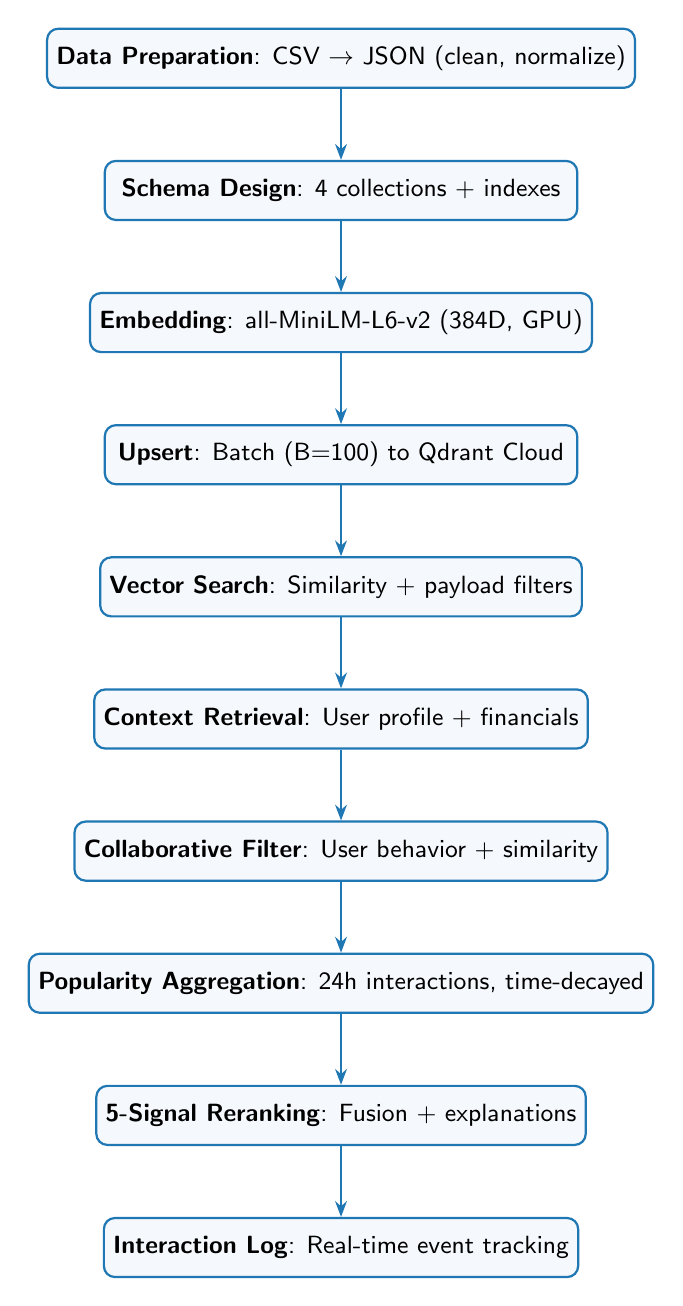
\begin{tikzpicture}[
  node distance=0.9cm,
  box/.style={rectangle, rounded corners, draw=accent, line width=0.8pt, align=center, minimum width=6cm, minimum height=0.75cm, fill=softbg, font=\small},
  arrow/.style={-{Stealth[length=2mm]}, thick, draw=accent}
]
  \node[box] (prep) {\textbf{Data Preparation}: CSV $\rightarrow$ JSON (clean, normalize)};
  \node[box, below=of prep] (schema) {\textbf{Schema Design}: 4 collections + indexes};
  \node[box, below=of schema] (embed) {\textbf{Embedding}: all-MiniLM-L6-v2 (384D, GPU)};
  \node[box, below=of embed] (upsert) {\textbf{Upsert}: Batch (B=100) to Qdrant Cloud};
  \node[box, below=of upsert] (search) {\textbf{Vector Search}: Similarity + payload filters};
  \node[box, below=of search] (context) {\textbf{Context Retrieval}: User profile + financials};
  \node[box, below=of context] (collab) {\textbf{Collaborative Filter}: User behavior + similarity};
  \node[box, below=of collab] (pop) {\textbf{Popularity Aggregation}: 24h interactions, time-decayed};
  \node[box, below=of pop] (rerank) {\textbf{5-Signal Reranking}: Fusion + explanations};
  \node[box, below=of rerank] (log) {\textbf{Interaction Log}: Real-time event tracking};
  
  \draw[arrow] (prep) -- (schema);
  \draw[arrow] (schema) -- (embed);
  \draw[arrow] (embed) -- (upsert);
  \draw[arrow] (upsert) -- (search);
  \draw[arrow] (search) -- (context);
  \draw[arrow] (context) -- (collab);
  \draw[arrow] (collab) -- (pop);
  \draw[arrow] (pop) -- (rerank);
  \draw[arrow] (rerank) -- (log);
\end{tikzpicture}
\caption{End-to-end system architecture and data flow}
\label{fig:architecture}
\end{figure}

\section{Qdrant Vector Database Design}

\subsection{Why Qdrant}

Traditional databases optimize for point-lookup and structured queries. Qdrant is purpose-built for \textit{vector-native memory}: storing, indexing, and querying high-dimensional embeddings at production scale.

Key advantages for FinCommerce:

\begin{enumerate}[leftmargin=1.2em]
  \item \textbf{Semantic Similarity at Scale}: Cosine similarity search finds products semantically related to user queries in sub-100ms on cloud instances, enabling real-time recommendation
  
  \item \textbf{Hybrid Search}: Payload filters on top of vector similarity allow simultaneous semantic and business-logic filtering (e.g., ``semantically similar AND price $\leq$ user capacity'')
  
  \item \textbf{Real-Time Updates}: Interactions logged at query-time are immediately upserted to Qdrant, making collaborative and popularity signals fresh without batch delays
  
  \item \textbf{Memory Efficiency}: Binary quantization and scalar quantization reduce disk/memory footprint while maintaining retrieval quality
  
  \item \textbf{Multi-Vector Support}: Collections can embed different semantic aspects (e.g., products via description, users via preference profile) enabling cross-modal discovery
\end{enumerate}

\subsection{Collections Design}

The system uses four specialized collections, each encoding different semantic aspects of the FinCommerce domain.

\subsubsection{Collection 1: products\_multimodal}

\begin{description}[labelwidth=2.5cm, leftmargin=3cm]
  \item[\textbf{Purpose}] Central product catalog with semantic embeddings of product descriptions
  
  \item[\textbf{Vector}] 384-dimensional embedding of product name, description, specs, and category via SentenceTransformer
  
  \item[\textbf{Semantic Meaning}] The vector encodes semantic intent: ``gaming laptop with RTX GPU under \$1500'' clusters near semantically similar products regardless of exact keyword matching
  
  \item[\textbf{Payload Fields}]
  \begin{itemize}
    \item product\_id (keyword indexed)
    \item name
    \item description
    \item categories[] (keyword indexed)
    \item brand (keyword indexed)
    \item price (numeric, filterable)
    \item in\_stock (boolean)
    \item image\_url
    \item currency
  \end{itemize}
  
  \item[\textbf{Distance Metric}] Cosine similarity (invariant to vector magnitude)
  
  \item[\textbf{Query Example}] User query ``laptop for ML under 1500'' is embedded; Qdrant returns top-K products with highest cosine similarity to query embedding, filtered by price $\leq$ 1500
\end{description}

\subsubsection{Collection 2: user\_profiles}

\begin{description}[labelwidth=2.5cm, leftmargin=3cm]
  \item[\textbf{Purpose}] User preference profiles encoding brand affinity, category preferences, and shopping persona
  
  \item[\textbf{Vector}] 384-dimensional embedding of aggregated user profile: ``prefers Apple and Dell; interested in Electronics, Computing; risk-tolerant; price-sensitive''
  
  \item[\textbf{Semantic Meaning}] The vector encodes user taste space: a user with Apple/premium preference clusters near other premium-brand enthusiasts, enabling user-based similarity
  
  \item[\textbf{Payload Fields}]
  \begin{itemize}
    \item user\_id (keyword indexed)
    \item location
    \item risk\_tolerance (0--1 scale)
    \item preferred\_categories[] (keyword indexed)
    \item preferred\_brands[] (keyword indexed)
    \item shopping\_frequency
    \item average\_order\_value
  \end{itemize}
  
  \item[\textbf{Distance Metric}] Cosine similarity
  
  \item[\textbf{Use Case}] Search collection to find users similar to a target user; boost products purchased by similar users in collaborative filtering
\end{description}

\subsubsection{Collection 3: financial\_contexts}

\begin{description}[labelwidth=2.5cm, leftmargin=3cm]
  \item[\textbf{Purpose}] Real-time financial state per user (balance, credit, debt, eligibility for installments)
  
  \item[\textbf{Vector}] 256-dimensional embedding of financial summary: ``balance \$800, credit \$1000, debt \$200, can afford installments''
  
  \item[\textbf{Semantic Meaning}] While less semantically rich than other collections, this vector captures financial feasibility space: users in similar financial situations cluster together, enabling financial affordability clustering
  
  \item[\textbf{Payload Fields}]
  \begin{itemize}
    \item user\_id (keyword indexed)
    \item available\_balance (numeric)
    \item credit\_limit (numeric)
    \item current\_debt (numeric)
    \item eligible\_installments (boolean)
    \item installment\_capacity (numeric)
    \item last\_updated (timestamp)
  \end{itemize}
  
  \item[\textbf{Distance Metric}] Cosine similarity
  
  \item[\textbf{Query Pattern}] Retrieve by user\_id; use payload fields for affordability scoring rather than vector search
\end{description}

\subsubsection{Collection 4: interaction\_memory}

\begin{description}[labelwidth=2.5cm, leftmargin=3cm]
  \item[\textbf{Purpose}] Real-time behavioral memory: every user interaction (view, click, add-to-cart, purchase) is logged with semantic and temporal context
  
  \item[\textbf{Vector}] 384-dimensional embedding of interaction context: ``user purchased MacBook Pro price 1299 for laptop ML category Electronics brand Apple''
  
  \item[\textbf{Semantic Meaning}] The vector encodes behavioral intent: what users buy/interact with. Similar users' interaction vectors surface collaborative signals
  
  \item[\textbf{Payload Fields}]
  \begin{itemize}
    \item user\_id (keyword indexed)
    \item product\_id (keyword indexed)
    \item interaction\_type (view, click, add\_to\_cart, purchase; keyword indexed)
    \item timestamp (numeric, indexed for time-decay filtering)
    \item weight (0.1 for view, 0.3 for click, 0.6 for cart, 1.0 for purchase)
    \item category (keyword indexed)
    \item brand (keyword indexed)
    \item price (numeric)
  \end{itemize}
  
  \item[\textbf{Distance Metric}] Cosine similarity
  
  \item[\textbf{Query Pattern}] Aggregate interactions by user\_id within a time window; construct user behavior vector from top-K interactions (weighted by recency decay); search for similar users' interactions
\end{description}

\subsection{Summary Table}

\begin{center}
\begin{tabular}{lllll}
\toprule
\textbf{Collection} & \textbf{Vector Dim} & \textbf{Distance} & \textbf{Primary Purpose} & \textbf{Key Indexed Field}\\
\midrule
products\_multimodal & 384 & Cosine & Product catalog semantics & product\_id, price\\
user\_profiles & 384 & Cosine & User preferences \& persona & user\_id\\
financial\_contexts & 256 & Cosine & Affordability context & user\_id\\
interaction\_memory & 384 & Cosine & Behavioral memory & user\_id, timestamp\\
\bottomrule
\end{tabular}
\end{center}

\section{Embedding \& Semantic Search}

\subsection{Embedding Model}

The system uses \textbf{SentenceTransformer (all-MiniLM-L6-v2)}:

\begin{itemize}[leftmargin=1.2em]
  \item \textbf{Model}: all-MiniLM-L6-v2 (384-dimensional output)
  \item \textbf{Training Data}: Trained on diverse sentence pairs (SBERT framework)
  \item \textbf{Strength}: Excellent semantic understanding at low computational cost; fast inference
  \item \textbf{Acceleration}: Automatic GPU detection (CUDA if available; CPU fallback)
  \item \textbf{Batch Processing}: Embeddings computed in batches (B=100) for throughput
\end{itemize}

\subsection{Vector Semantics}

A 384-dimensional vector is not human-interpretable in isolation, but its \textit{position in embedding space} encodes semantic meaning:

\begin{enumerate}[leftmargin=1.2em]
  \item \textbf{For Products}: The vector encodes product semantics. A query ``gaming laptop'' and a product ``high-performance gaming laptop with RTX 3080'' have high cosine similarity because their semantic content overlaps.
  
  \item \textbf{For Users}: The vector encodes preference semantics. A user interested in ``Apple, Electronics, premium brands'' clusters near other premium-brand enthusiasts.
  
  \item \textbf{For Interactions}: The vector encodes behavioral semantics. An interaction ``user purchased expensive electronics'' clusters near other similar users' interactions.
\end{enumerate}

\subsection{Similarity Search}

Query processing follows this workflow:

\begin{enumerate}[leftmargin=1.2em]
  \item \textbf{Embed User Query}: Natural-language query string is passed through SentenceTransformer to produce 384D vector (e.g., ``laptop for machine learning under 1500'' $\rightarrow$ $v_q \in \mathbb{R}^{384}$)
  
  \item \textbf{Vector Search}: Query vector is sent to Qdrant with payload filter (e.g., price $\leq$ user capacity). Qdrant returns top-K products ranked by cosine similarity.
  
  \item \textbf{Similarity Metric}: 
  \[
    \text{cosine\_similarity}(v_q, v_p) = \frac{v_q \cdot v_p}{\|v_q\|_2 \|v_p\|_2}
  \]
  Scores range in $[-1, 1]$, normalized to $[0, 1]$ for downstream fusion.
  
  \item \textbf{Top-K Retrieval}: Typically K=100; these products are passed to reranking pipeline (see Section \ref{sec:scoring}).
\end{enumerate}

\subsection{Performance}

\begin{center}
\begin{tabular}{ll}
\toprule
\textbf{Operation} & \textbf{Latency}\\
\midrule
Embedding (single query, GPU) & 40--60 ms\\
Embedding (single query, CPU) & 120--200 ms\\
Qdrant vector search (top-100) & 100--150 ms\\
Payload filtering & 20--50 ms\\
\bottomrule
\end{tabular}
\end{center}

\section{Scoring \& Ranking Strategy}
\label{sec:scoring}

The system combines five independent scoring signals into a unified ranking via weighted fusion. Each signal captures a different dimension of product suitability.

\subsection{Signal 1: Semantic Score ($s_{\text{sem}}$)}

\begin{description}[labelwidth=3.5cm, leftmargin=4cm]
  \item[\textbf{Definition}] Cosine similarity between user query embedding and product embedding, directly from Qdrant vector search
  
  \item[\textbf{Interpretation}] Measures how semantically relevant the product is to the user's stated intent
  
  \item[\textbf{Range}] $s_{\text{sem}} \in [0, 1]$ (normalized from $[-1, 1]$)
  
  \item[\textbf{Example}] Query ``gaming laptop with RTX'' has $s_{\text{sem}} = 0.92$ for ``ASUS TUF Gaming A16 with RTX 4090'' and $s_{\text{sem}} = 0.45$ for ``Office tablet''
  
  \item[\textbf{Weight in Fusion}] 0.30 (highest weight—semantic relevance is table stakes)
\end{description}

\subsection{Signal 2: Affordability Score ($s_{\text{aff}}$)}

\begin{description}[labelwidth=3.5cm, leftmargin=4cm]
  \item[\textbf{Definition}] Function of product price relative to user financial capacity
  
  \item[\textbf{Formula}]
  \[
    s_{\text{aff}} = \max\left(0, 1 - \frac{\text{price}}{\text{balance} + \text{credit\_limit}}\right)
  \]
  
  \item[\textbf{Interpretation}] Products with price $\leq$ (balance + credit\_limit) receive positive scores; more expensive items are penalized proportionally but not eliminated (graceful degradation)
  
  \item[\textbf{Example}]
  \begin{itemize}
    \item User: balance=\$800, credit\_limit=\$1000, total capacity=\$1800
    \item Product A: price=\$900 $\Rightarrow$ $s_{\text{aff}} = 1 - \frac{900}{1800} = 0.50$
    \item Product B: price=\$1800 $\Rightarrow$ $s_{\text{aff}} = 1 - \frac{1800}{1800} = 0.00$
    \item Product C: price=\$2500 $\Rightarrow$ $s_{\text{aff}} = \max(0, 1 - \frac{2500}{1800}) = 0.00$ (same as limit-hitting)
  \end{itemize}
  
  \item[\textbf{Weight in Fusion}] 0.25 (second highest—affordability is non-negotiable in FinCommerce)
\end{description}

\subsection{Signal 3: Preference Score ($s_{\text{pref}}$)}

\begin{description}[labelwidth=3.5cm, leftmargin=4cm]
  \item[\textbf{Definition}] Alignment between product attributes (brand, categories) and user preferences
  
  \item[\textbf{Formula}]
  \[
    s_{\text{pref}} = \max\left(\frac{|\text{user\_brands} \cap \{\text{product\_brand}\}|}{|\text{user\_brands}|}, \frac{|\text{user\_cats} \cap \text{product\_cats}|}{|\text{user\_cats}|}\right)
  \]
  
  \item[\textbf{Interpretation}] If product brand is in user's preferred brands list OR product categories overlap with user's favorite categories, score $> 0$. Score increases with match ratio
  
  \item[\textbf{Example}]
  \begin{itemize}
    \item User preferred brands: \{Apple, Dell\}, preferred categories: \{Electronics, Computing\}
    \item Product A: brand=Apple, categories=\{Electronics\} $\Rightarrow$ $s_{\text{pref}} = \max(1/2, 1/2) = 0.50$
    \item Product B: brand=Sony, categories=\{Electronics, Audio\} $\Rightarrow$ $s_{\text{pref}} = \max(0, 1/2) = 0.50$
    \item Product C: brand=Shein, categories=\{Fashion\} $\Rightarrow$ $s_{\text{pref}} = \max(0, 0) = 0.00$
  \end{itemize}
  
  \item[\textbf{Weight in Fusion}] 0.15 (moderate weight—preference is important but secondary to relevance and affordability)
\end{description}

\subsection{Signal 4: Collaborative Score ($s_{\text{collab}}$)}

\begin{description}[labelwidth=3.5cm, leftmargin=4cm]
  \item[\textbf{Definition}] How much similar users have interacted with or purchased this product
  
  \item[\textbf{Algorithm}]
  \begin{enumerate}
    \item Construct user behavior vector $b_u$ from target user's last 10 interactions, weighted by recency (7-day decay):
    \[
      b_u = \sum_{i=1}^{10} w_i \cdot e^{-\lambda_{\text{collab}} \Delta t_i} \cdot v_{i,\text{interaction}}
    \]
    where $\lambda_{\text{collab}} = \ln(2) / (7 \times 86400)$ (7-day half-life)
    
    \item Search interaction\_memory collection for similar user interactions (exclude self)
    
    \item Aggregate weighted interactions on target product:
    \[
      s_{\text{collab}} = \frac{\sum_{j \in \text{similar users}} \text{similarity}(b_u, b_j) \cdot w_j}{\max(\text{all collaborative aggregates})}
    \]
  \end{enumerate}
  
  \item[\textbf{Interpretation}] Users who are behaviorally similar to the target user and who have purchased/clicked/viewed this product boost the product's score
  
  \item[\textbf{Weight in Fusion}] 0.20 (second-highest weight—collaborative signals are powerful for discovery)
\end{description}

\subsection{Signal 5: Popularity Score ($s_{\text{pop}}$)}

\begin{description}[labelwidth=3.5cm, leftmargin=4cm]
  \item[\textbf{Definition}] Time-decayed aggregation of user interactions (views, clicks, purchases) on product in past 24 hours
  
  \item[\textbf{Algorithm}]
  \begin{enumerate}
    \item Query interaction\_memory for all interactions on target product\_id with timestamp within 24 hours
    
    \item For each interaction, apply weight (view=0.1, click=0.3, cart=0.6, purchase=1.0) and exponential time decay:
    \[
      \text{score}_j = w_{\text{type}} \cdot e^{-\lambda_{\text{pop}} (t_{\text{now}} - t_j)}
    \]
    where $\lambda_{\text{pop}} = \ln(2) / (6 \times 3600)$ (6-hour half-life)
    
    \item Aggregate:
    \[
      s_{\text{pop}} = \frac{\sum_j \text{score}_j}{\max(\text{all popularity aggregates})}
    \]
  \end{enumerate}
  
  \item[\textbf{Interpretation}] Products with recent, numerous, weighted interactions (purchases $>$ carts $>$ clicks $>$ views) receive high popularity scores. Importance decays exponentially; interactions older than 24 hours contribute zero.
  
  \item[\textbf{Example}]
  \begin{itemize}
    \item Product A: 1 purchase 30 min ago, 5 clicks 2 hours ago $\Rightarrow$ high $s_{\text{pop}}$
    \item Product B: 50 views 20 hours ago, no recent interactions $\Rightarrow$ very low $s_{\text{pop}}$
  \end{itemize}
  
  \item[\textbf{Weight in Fusion}] 0.10 (lowest weight—popularity is a tiebreaker, not primary driver)
\end{description}

\subsection{Final Ranking Formula}

The five signals are combined via weighted linear fusion:

\[
  \text{final\_score} = 0.30 \cdot s_{\text{sem}} + 0.25 \cdot s_{\text{aff}} + 0.15 \cdot s_{\text{pref}} + 0.20 \cdot s_{\text{collab}} + 0.10 \cdot s_{\text{pop}}
\]

All component scores are normalized to $[0, 1]$ before fusion. Products are ranked by final\_score in descending order.

\subsection{Rationale for Weights}

\begin{enumerate}[leftmargin=1.2em]
  \item \textbf{Semantic (0.30)}: User explicitly stated intent must be respected; semantic irrelevance cannot be overcome by other signals
  
  \item \textbf{Affordability (0.25)}: In FinCommerce, recommending unaffordable items damages trust; affordability is nearly co-equal with relevance
  
  \item \textbf{Collaborative (0.20)}: Behavioral signals are powerful for discovery; similar users' purchases identify non-obvious relevant items
  
  \item \textbf{Preference (0.15)}: User preferences matter but are secondary to relevance and affordability; low-preference items can still rank high if highly relevant and affordable
  
  \item \textbf{Popularity (0.10)}: Trending items are valuable for awareness but risk recommending fads; used as a tiebreaker among otherwise equal alternatives
\end{enumerate}

\section{Real-Time Interaction Learning}

Unlike batch-trained recommendation systems that update offline, this engine learns from user interactions in real-time, enabling immediate personalization and trend detection.

\subsection{Interaction Types \& Weights}

Every user action is captured with semantic and temporal context:

\begin{center}
\begin{tabular}{llll}
\toprule
\textbf{Interaction Type} & \textbf{User Intent} & \textbf{Weight} & \textbf{Trigger}\\
\midrule
View & Awareness, curiosity & 0.1 & Product displayed in search results\\
Click & Consideration, interest & 0.3 & User clicks product card\\
Add-to-Cart & High intent, evaluation & 0.6 & User adds to cart\\
Purchase & Commitment, satisfaction & 1.0 & User completes purchase\\
\bottomrule
\end{tabular}
\end{center}

The weight progression (0.1 $\rightarrow$ 0.3 $\rightarrow$ 0.6 $\rightarrow$ 1.0) reflects purchase funnel depth: purchases are 10x more informative than passive views.

\subsection{Interaction Logging Mechanism}

\begin{enumerate}[leftmargin=1.2em]
  \item \textbf{Capture}: User action triggers event in Streamlit UI
  
  \item \textbf{Enrich}: Interaction is augmented with product metadata (brand, category, price) and user context (user\_id, timestamp)
  
  \item \textbf{Embed}: Interaction summary is embedded via SentenceTransformer:
  \begin{quote}
    ``User [action] [product name] price [price] category [category] brand [brand]''
  \end{quote}
  E.g., ``User purchased MacBook Pro 16-inch price 2499 category Electronics brand Apple''
  
  \item \textbf{Upsert}: Interaction vector + payload are upserted to interaction\_memory collection in Qdrant (latency $< 50$ms)
  
  \item \textbf{Immediate Impact}: Future queries by this user or similar users immediately incorporate the new interaction via collaborative and popularity scoring
\end{enumerate}

\subsection{Popularity vs.\ Collaborative Filtering}

Both signals use interaction\_memory but in different ways:

\begin{description}[labelwidth=3cm, leftmargin=3.5cm]
  \item[\textbf{Popularity}] Aggregates interactions on a single product across all users, weighted by recency. Answers: ``Is this product trending right now?'' Used to surface emerging items and detect temporary spikes in interest.
  
  \item[\textbf{Collaborative}] Aggregates interactions by user, computes user similarity, then finds products purchased by similar users. Answers: ``What did people like me buy?'' Used for personalized discovery based on past behavior.
\end{description}

\subsection{Time Decay Rationale}

\begin{enumerate}[leftmargin=1.2em]
  \item \textbf{Collaborative Decay (7-day half-life)}: User preferences evolve slowly. Purchases from 7 days ago are still relevant for inferring taste, but weighted at 50\% influence. Purchases from 14 days ago have 25\% influence. This balances freshness with stability.
  
  \item \textbf{Popularity Decay (6-hour half-life)}: Trends move fast. A product gaining attention in the last 6 hours is immediately boosted; after 12 hours it has half the score; after 24 hours it has negligible influence. This captures viral moments without stale ranking.
\end{enumerate}

\section{Explainability Layer}

Recommendations without explanations erode user trust. Each ranked product includes structured, human-readable explanations across five categories.

\subsection{Explanation Framework}

For each product in final ranking, the system generates explanations from each of the five signals:

\subsubsection{1. Semantic Relevance Explanation}

Based on semantic score:
\begin{itemize}[leftmargin=1.2em]
  \item Score $\geq 0.85$: ``Strong match to your search query [query terms]''
  \item Score 0.70--0.84: ``Closely matches your search [query terms]''
  \item Score 0.50--0.69: ``Related to your search for [query terms]''
  \item Score $< 0.50$: ``Loosely related to your search''
\end{itemize}

\subsubsection{2. Affordability Explanation}

Based on affordability score and price relative to capacity:
\begin{itemize}[leftmargin=1.2em]
  \item Price $\leq$ balance: ``Well within your available balance''
  \item Price $\leq$ balance + credit\_limit: ``Fits within your total financial capacity''
  \item Price $>$ capacity but score $> 0$: ``Stretches your budget but may be eligible for installments''
  \item Price far exceeds: ``Currently outside your financial reach''
\end{itemize}

\subsubsection{3. Preference Explanation}

Based on preference score:
\begin{itemize}[leftmargin=1.2em]
  \item Perfect match: ``Matches your preferred brand: [brand]''
  \item Category match: ``In your favorite category: [category]''
  \item Partial match: ``Related to your interests''
  \item No match: ``New to your preferences''
\end{itemize}

\subsubsection{4. Collaborative Explanation}

Based on collaborative score:
\begin{itemize}[leftmargin=1.2em]
  \item High score: ``Similar users purchased this recently''
  \item Moderate score: ``Popular among users with your preferences''
  \item Low score: ``Some similar users have viewed this''
  \item Zero score: ``New product, no user signals yet''
\end{itemize}

\subsubsection{5. Popularity Explanation}

Based on popularity score and interaction count:
\begin{itemize}[leftmargin=1.2em]
  \item High activity: ``Very popular in last 24 hours ([N] interactions)''
  \item Moderate activity: ``Getting attention this week''
  \item Low activity: ``Steady interest from users''
  \item No activity: ``Not currently trending''
\end{itemize}

\subsection{Benefits}

Structured explanations provide:

\begin{enumerate}[leftmargin=1.2em]
  \item \textbf{Transparency}: Users understand why they see each product, building trust
  
  \item \textbf{Discoverability}: Users learn what signals drive recommendations, enabling better queries
  
  \item \textbf{Refinement}: Users can ignore products if explanations don't align with intent (e.g., ``You said you wanted under \$1000 but this is \$1200'')
  
  \item \textbf{Debugging}: System designers can audit ranking decisions by examining explanations
\end{enumerate}

\section{User Interface}

The Streamlit-based web interface enables users to explore products, log interactions, and see recommendations with full explainability.

\subsection{Interface Sections}

\subsubsection{Sidebar: Context Configuration}

Users configure search context:

\begin{itemize}[leftmargin=1.2em]
  \item \textbf{User Selection}: Dropdown to select user (simulates multi-user environment)
  
  \item \textbf{Budget Input}: Slider for max price filter (0--5000)
  
  \item \textbf{Financial Context Display}: Shows available balance, credit limit, total capacity (read-only, for transparency)
  
  \item \textbf{Preference Display}: Lists preferred brands and categories (read-only)
\end{itemize}

\subsubsection{Main Panel: Search \& Results}

\begin{enumerate}[leftmargin=1.2em]
  \item \textbf{Query Input}: Text box for natural-language product query (e.g., ``laptop for machine learning'')
  
  \item \textbf{Search Button}: Executes search pipeline; displays results ranked by final\_score
  
  \item \textbf{Results Display}: For each product:
  \begin{itemize}
    \item Product name, brand, price, in-stock status
    \item Final score (0--1 bar visualization)
    \item Structured multi-reason explanations (icons + text from each signal)
    \item Interactive buttons: ``View Details'', ``Add to Cart'', ``Mark as Purchased''
  \end{itemize}
  
  \item \textbf{Interaction Tracking}: Clicking any button triggers interaction logger, immediately updating Qdrant and influencing future recommendations
\end{enumerate}

\subsection{Real-Time Feedback}

\begin{enumerate}[leftmargin=1.2em]
  \item \textbf{Logging Confirmation}: Toast notification confirms interaction logged (``Interaction recorded'')
  
  \item \textbf{Score Refresh}: After logging an interaction, if the same product appears in a future search, users see updated collaborative/popularity scores
  
  \item \textbf{Trending Updates}: If a product receives a purchase during a session, its popularity score immediately increases, influencing other users' queries
\end{enumerate}

\section{Scalability \& Extensibility}

The architecture is designed for production deployment and future enhancements.

\subsection{Scalability Dimensions}

\subsubsection{Vertical Scaling: More Data}

\begin{enumerate}[leftmargin=1.2em]
  \item \textbf{Products}: Current system handles 50K--500K products; Qdrant scales to millions with pagination
  
  \item \textbf{Users}: Interaction logging is sub-linear; millions of users supported
  
  \item \textbf{Interactions}: Interaction\_memory collection can aggregate 1M+ interactions with time-window filtering; Qdrant's indexing remains sub-second
\end{enumerate}

\subsubsection{Horizontal Scaling: Distributed Deployment}

\begin{enumerate}[leftmargin=1.2em]
  \item \textbf{Qdrant Cluster}: Qdrant Cloud supports replication and sharding; read-heavy queries (search) are horizontally distributed
  
  \item \textbf{Embedding Service}: SentenceTransformer inference can be containerized (Docker) and deployed on multiple GPUs in Kubernetes
  
  \item \textbf{Search Pipeline}: Stateless Python backend (Flask/FastAPI) can run in multiple replicas; load balancer distributes queries
\end{enumerate}

\subsection{Extensibility}

\subsubsection{Multi-Modal Embeddings}

Current system embeds text descriptions. Future enhancements:

\begin{itemize}[leftmargin=1.2em]
  \item \textbf{Image Embeddings}: Use CLIP or similar to embed product images; enable visual search (``show me products similar to this image'')
  
  \item \textbf{Fusion}: Combine text embeddings (SentenceTransformer) with image embeddings; improve semantic understanding
\end{itemize}

\subsubsection{Cross-Domain Catalog}

Currently limited to 4 e-commerce datasets. Extensions:

\begin{itemize}[leftmargin=1.2em]
  \item \textbf{Real Estate}: Embed properties by description; enable ``find me homes under \$500K with my preferred neighborhood''
  
  \item \textbf{Job Search}: Embed job descriptions and candidate profiles; enable ``find me roles matching my skills under my salary expectation''
  
  \item \textbf{Travel}: Embed destinations and budgets; enable ``find me vacations under \$2000 with my preferred activities''
\end{itemize}

\subsubsection{Advanced Collaboration}

Current collaborative filtering is user-based. Future enhancements:

\begin{itemize}[leftmargin=1.2em]
  \item \textbf{Item-Based CF}: Cluster products via interaction vectors; recommend ``products frequently bought together''
  
  \item \textbf{Deep Learning CF}: Train neural collaborative filtering models on interaction history for more expressive patterns
  
  \item \textbf{Context-Aware CF}: Incorporate time-of-day, season, user mood (via query analysis) into collaborative scores
\end{itemize}

\subsection{Production Readiness}

The system includes infrastructure for production deployment:

\begin{enumerate}[leftmargin=1.2em]
  \item \textbf{Comprehensive Logging}: All API calls, embeddings, searches, and interactions logged to files and monitoring dashboards
  
  \item \textbf{Error Handling}: Graceful degradation (e.g., if Qdrant is down, fall back to keyword search; if collaborative filtering fails, use semantic + affordability only)
  
  \item \textbf{Performance Monitoring}: Latency tracking for embedding, search, and ranking; alerts if any stage exceeds thresholds
  
  \item \textbf{A/B Testing}: Framework for comparing ranking formulas, weights, and algorithms before deploying to production
  
  \item \textbf{Cold Start}: New users, new products, new categories handled gracefully; no recommendations withheld due to missing signals
\end{enumerate}

\section{Conclusion}

The Context-Aware FinCommerce Engine demonstrates how vector databases fundamentally transform e-commerce personalization. By embedding all entities—products, users, financial states, and behavioral interactions—into a unified semantic space, we enable sub-second hybrid retrieval that simultaneously reasons over semantic intent, financial feasibility, personal preferences, collaborative signals, and real-time trends.

Key innovations:

\begin{enumerate}[leftmargin=1.2em]
  \item \textbf{Vector-Native Memory}: Qdrant serves as the central intelligence layer, eliminating the need for separate search engines, recommendation services, and trend trackers
  
  \item \textbf{Real-Time Personalization}: Every user interaction immediately influences recommendations for that user and similar users; no batch delays
  
  \item \textbf{Financial Intelligence}: Affordability scoring explicitly encodes financial constraints, ensuring recommendations respect user capacity
  
  \item \textbf{Explainability}: Multi-reason explanations provide transparency and enable user refinement
  
  \item \textbf{Production Architecture}: Comprehensive logging, error handling, and monitoring ensure reliability at scale
\end{enumerate}

The system is immediately applicable to any vertical where users have budget constraints and benefit from personalization: e-commerce, travel, real estate, job boards, lending, and beyond. It demonstrates that vector intelligence is not a future technology—it is a present-day competitive advantage in recommendation systems.

\end{document}
